De Computer Management\index{computer management console}\index{mmc!computer management console} (Computerbeheer\index{computerbeheer}\index{mmc!computerbeheer}) console is een Microsoft Management Console (MMC) snap-in die voorziet in een aantal zaken voor het beheer van systeem componenten, services en settings voor Windows. Binnen Computer Management kan je o.a. de disk, services en shared folders beheren. Daarnaast zijn er nog vele andere beheertaken die er gedaan kunnen worden.

Om Computer Management te openen zijn er verschillende manieren:
\begin{itemize}
\item
	\begin{enumerate}
		\item Start MMC
		\item Selecteer in het File menu Add/Remove snap-in
		\item Selecteer Computer Management en klik op Add
		\item Voor de lokale machine selecteer Finish
	\end{enumerate}
\item Gebruik de windows-toets + r en run compmgmt.msc\index{compmgmt.msc}
\item Klik op het zoek icoon en zoek op Computer Management
\end{itemize}

\begin{minipage}[t]{\linewidth}
\raggedright
\adjustbox{valign=t}{%
	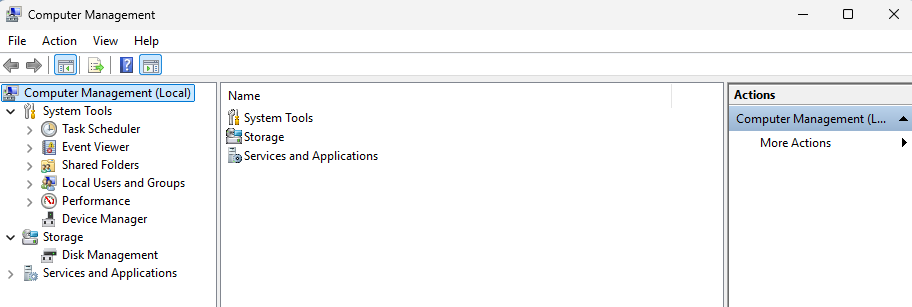
\includegraphics[width=0.99\linewidth]{computermanagement.png}%
}
\end{minipage}

